%%
%% This is file `mcmthesis-demo.tex',
%% generated with the docstrip utility.
%%
%% The original source files were:
%%
%% mcmthesis.dtx  (with options: `demo')
%%
%% -----------------------------------
%%
%% This is a generated file.
%%
%% Copyright (C)
%%       2010 -- 2015 by Zhaoli Wang
%%       2014 -- 2019 by Liam Huang
%%       2019 -- present by latexstudio.net
%%
%% This work may be distributed and/or modified under the
%% conditions of the LaTeX Project Public License, either version 1.3
%% of this license or (at your option) any later version.
%% The latest version of this license is in
%%   http://www.latex-project.org/lppl.txt
%% and version 1.3 or later is part of all distributions of LaTeX
%% version 2005/12/01 or later.
%%
%% This work has the LPPL maintenance status `maintained'.
%%
%% The Current Maintainer of this work is Liam Huang.
%%
%%
%% This is file `mcmthesis-demo.tex',
%% generated with the docstrip utility.
%%
%% The original source files were:
%%
%% mcmthesis.dtx  (with options: `demo')
%%
%% -----------------------------------
%%
%% This is a generated file.
%%
%% Copyright (C)
%%       2010 -- 2015 by Zhaoli Wang
%%       2014 -- 2019 by Liam Huang
%%       2019 -- present by latexstudio.net
%%
%% This work may be distributed and/or modified under the
%% conditions of the LaTeX Project Public License, either version 1.3
%% of this license or (at your option) any later version.
%% The latest version of this license is in
%%   http://www.latex-project.org/lppl.txt
%% and version 1.3 or later is part of all distributions of LaTeX
%% version 2005/12/01 or later.
%%
%% This work has the LPPL maintenance status `maintained'.
%%
%% The Current Maintainer of this work is Liam Huang.
%%
\documentclass{mcmthesis}
\mcmsetup{CTeX = false,   % 使用 CTeX 套装时,设置为 true
        tcn = 2013083, problem = F,
        sheet = true, titleinsheet = false, keywordsinsheet = true,
        titlepage = true, abstract = true}
\usepackage{newtxtext}%\usepackage{palatino}
\usepackage{lipsum}
\usepackage{float}
\usepackage{graphicx}
\usepackage{subfigure}
\newcommand{\upcite}[1]{\textsuperscript{\textsuperscript{\cite{#1}}}} 
\title{How Should the UN Respond for EDPs}%标题
\date{\today}
\begin{document}
\begin{abstract}
	
In order to study the EDPs problem and propose effective policies, taking the principle of economics and game theory as the core, this paper constructed a policy establishment system including the models of EDPs size prediction, cultural risk assessment and communication simulation and policy formulation.Then we extended it further through Bayesian network.

First, the time series of sea level height was analyzed.And the scale of EDPs was predicted by combining the population growth rate of each country, the area of coastal areas and the altitude.
Later, the factors affecting the risk of cultural loss before and after migration were taken into special consideration by using the grey relational analysis system after selecting typical emigrating countries and migrating countries. Based on this, the cellular automation algorithm was used to simulate the cultural exchange process to express the evolution trend of cultural blending in the form of scatter plot.

The policy development model was the focus of this paper. A two-stage sequential game was established to predict the behavior of EDPs groups and receiving countries. At the same time, this paper also explored the perspectives that the UN policy should cut into. The benefits and the cost of receiving countries were divided into more specific and quantifiable parts. And the environmental protection index was measured to develop a mandatory reception ratio indicator. Then, the situation that may occur between the EDPs group and the receiving country was analyzed.

Finally, the Bayesian network was used to evaluate the policy arrangement with the goal of maximizing the expected return of the three parties after implementation of the policy. We also analysed how the UN should plan migration patterns in different periods by studying the examples of potential receiving countries. At last, it was found that the UN policies can indeed improve the efficiency of EDPs migration, eliminate certain potential conflicts, and lead to more harmonious global development.
Key words:policy formulation, sequential game, Bayesian network
\begin{keywords}
EDPs; cultural loss; policy formulation; sequential game; Bayesian network
\end{keywords}
\end{abstract}
\maketitle
%% Generate the Table of Contents, if it's needed.
\tableofcontents
\newpage
%%
%% Generate the Memorandum, if it's needed.
%% \memoto{\LaTeX{}studio}
%% \memofrom{Liam Huang}
%% \memosubject{Happy \TeX{}ing!}
%% \memodate{\today}
%% \logo{\LARGE I'm pretending to be a LOGO!}
%% \begin{memo}[Memorandum]
%%   \lipsum[1-3]
%% \end{memo}
%%
\section{Introduction}
\subsection{Background}

Due to the sea level rise and land degradation caused by global climate change, tens of millions or even hundreds of millions of people will be forced to leave their homes and head for strange areas. For example, Tuvalu, an island country in the Pacific Ocean, began its national migration several years ago. Besides, reports such as “Maldives is sinking to the bottom of the sea” are accustomed. With the reality factors interwoven with media rendering, the term "environmental refugee" is not too strange to us today.

The discussion about environmental refugees is getting more and more intense. Fom the perspective of EDPs, the concept of EDPs is different from that of refugees in the traditional sense, so most of the policies and documents issued by the world organization cannot be effectively applied to this group, which brings certain challenges to the survival of them and the protection of basic human rights.Fom the perspective of national machinery and international organizations, it is very likely that millions of people will migrate across national borders in this century, which may lead to the growth of conflicts among civilizations and produce negative effects on international peace. Based on these considerations, people believe that programs and policies that are in line with the current situation should be put forward as soon as possible to achieve the ultimate goal of stabilizing the international order and harmonious global development.

However, it is not easy to find feasible and acceptable programs and policies. The EDPs will bring a multi-subject international problem. The wishes of both the EDPs themselves and the receiving countries cannot be ignored. 

\subsection{Statment of the problem}
Problem F in the ICM requires us to serve as a policy analysis team and make effective policy recommendations to the United Nations on the issue of EDPs. 

First, we must clarify the scale of EDPs in the future. EDPs' groups of different scale will cause different degrees of economic and cultural shocks to the receiving countries. We collected the average altitude and population growth data of some countries that are most likely to suffer natural disasters in the future. Combined with the rise of sea level, we forecasted the number of EDPs through time series fitting and regression analysis. Second, we assessed the cultural differences between the countries where EDPs originally located and the receiving countries. Based on this we derived the risk of losing their culture after migration, which can be used as a reference for their choice of migration destination. Then, from the perspective of the respective interests of EDPs, receiving countries, and the United Nations, we put forward policy recommendations for EDPs. We assume that these three have their own interests to measure. EDPs and receiving countries make decisions based on their own interests. The UN, while making uncompromising rules for countries based on indicators such as greenhouse gas emissions, also making preferential policies to encourage countries to take EDPs. Finally, we use the Bayesian network to establish a policy benefit evaluation model, and simulate the process of cultural integration and transformation over a period of time.

\section{Components of the model}
Our model analyzes the situation of EDPs from multiple perspectives.Based on the analysis of the problem, we split the model into the following three parts:
\begin{enumerate}
\item Measuring the scope of people at risk 
\item The risk of loss of culture
\item Proposal of policies
\end{enumerate}
\section{Measuring the scope of People at risk}

Consider the cause of EDPs: the islands in which they live are at risk of disappearing due to rising sea levels. Based on the data of altitude of coastal lands and islands,this model takes the velocity of sea level's rise and the population growth into research domain.
\subsection{Prediction of sea level rise}

As a basis for predicting the number of EDPs over the next period of time, we conducted a time series analysis of sea level height in conjunction with known sea level altitude data for more than a hundred years ,and give the forecast value to 2050 based on this.

First, we observe the given data in order to have an intuitive understanding of the longitudinal data.After visualizating,we get a graph which illstrates that the sea level is generally on the rise, with little volatility.
\begin{figure}[H]%并列图片
	\begin{minipage}[t]{0.5\textwidth}
		\centering
		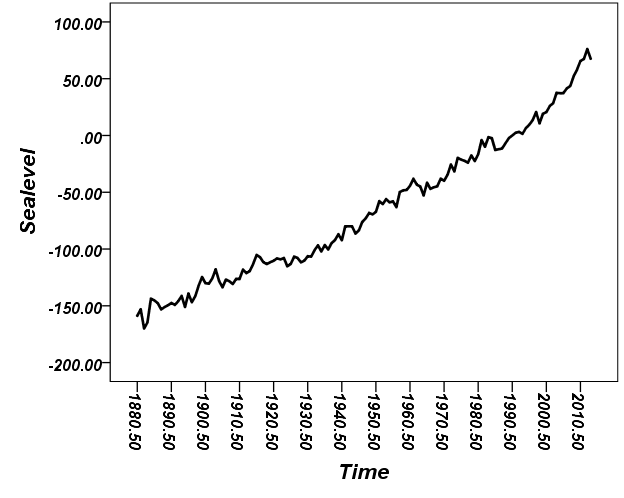
\includegraphics[scale=0.51]{haipingmianshijianxulietu}
		\caption{Sea level time series\label{fig:1}}
	\end{minipage}
	\qquad
	\begin{minipage}[t]{0.5\textwidth}
		\centering
		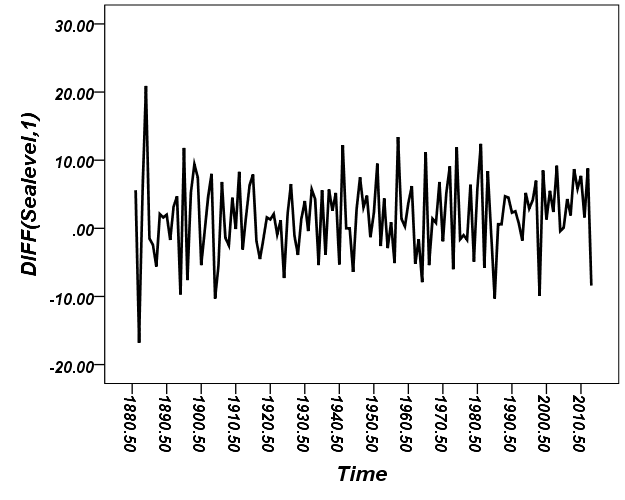
\includegraphics[scale=0.25]{haipingmianyijiechafen}
		\caption{First-order difference in sea level\label{fig:2}}
	\end{minipage}
\end{figure}

It has some stability and no additional cyclical changes in the trendency. Therefore, we consider that the time series analysis should meet the following requirements:
\begin{enumerate}
\item The fitted model should be able to represent the basic trend of the time series;
\item The model should have parameters to capture small range of fluctuations.
\end{enumerate}

Based on the above considerations, we propose the following formula:
\begin{equation}%公式
Z(t)=h(t)+s(t)
\end{equation}

Where  $ h(t) $ is the trend value, $ s(t) $ is the time-independent random noise. Processing the height data on sea level with a first-order differential, the results are shown in Figure2. It shows that the first-order difference of sea level height has good randomness and no obvious upward or downward trend. After using descriptive statistics methods, we also found that the frequency function is close to the normal distribution. The relatively strong fluctuations of the early stage, combined with reality, may be due to the limited measurement technology, inaccurate measurement results and other man-made factors. We then performed a self-correlation and partial correlation analysis of sea level data, and the results are as shown in Appendix A

%%这差个公式
\begin{equation}
\hat{p_{k}}=\dfrac{\sum_{n=1}^{n-k}(Z_{t}-\bar{Z})(Z_{t+k}-\bar{Z})}{\sum_{t=1}^{n}(Z_{t}-\bar{Z})^2}
\end{equation}
\begin{equation}
P_{k}=\dfrac{Cov[(Z_{t}-\hat{Z_{t}}),(Z_{t+K}-\hat{Z_{t+k}})]}{\sqrt{Var(Z_{t}-\hat{Z_{t}})}\sqrt{Var(Z_{t+k}-\hat{Z_{t+k}})}分母}
\end{equation}

The AMIRA method was then used to predict sea level altitude over a period of time, with the results shown in figure5.  It can be observed that the sea level has steadily increased from now on until 2050, as it has maintained a similar general trend for a long time. At the same time, considering the possible fluctuations, Figure6 gives the upper and lower limits of the 95\% confidence interval. All these indicate the long-term stability of sea level changes and the reliability of our predictions. 
\begin{figure}[h]%图片
	\small
	\centering
	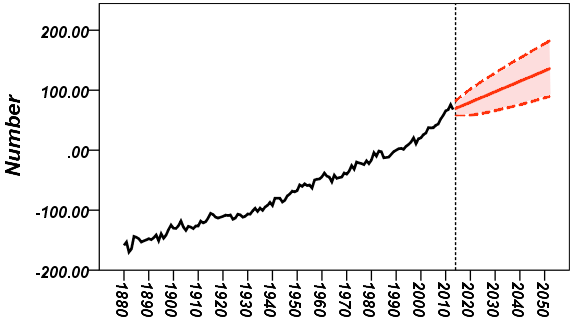
\includegraphics[width=8cm]{zongtixulie}%图片名
	\caption{Sea level height prediction} \label{fig:5}%题注
\end{figure}
\subsection{Prediction of the number of EDPs}
In this section, we analyse the impact of rising sea levels on the number of environmental refugees.
To simplify the model, we introduce the following assumptions:
\begin{enumerate}
\item Sea level rises at the same rate in all regions of the world, and will not change unevenly due to tidal effects or other factors.
\item The erosion of land by sea level rise does not need to wait until the sea level is as high as land. As long as the difference between them is reduced to a certain range, people on this part of the land risk not living normally. When the risk reaches a certain extent. Although the land has not been completely submerged by sea level, the people on it will still be forced to move and become EDPs.
\item The population growth rate remains unchanged.
\item Neglecting the time of the migration process, the number of environmental refugees will not decrease due to long distances or other factors.
\end{enumerate}

After looking for the data, we found that in addition to the long-term trend of sea level, the high and low tides in one day are also factors that cannot be ignored. According to data from different regions of the world, the tidal range ranges from 0m to 16.3m. Let the sea level height $ Z_{0}(t) $ obtained from the model in section 2.2 be the height of the flat tide. After fully considering the safety factors, we have reached the following two conclusions:

It should be obvious that all people living at altitudes within $ U_{1}=(Z_{0}(t), Z_{0}(t)+2) $should be relocated;
The population living at an altitude within $ U_{2}=(Z_{0}(t)+2, Z_{0}(t)+8) $ shall migrate according to a certain proportion.
Considering that the migration ratio obviously becomes smaller as the altitude increases, we established the following proportional function:

\begin{figure}[h]%图片
	\small
	\centering
	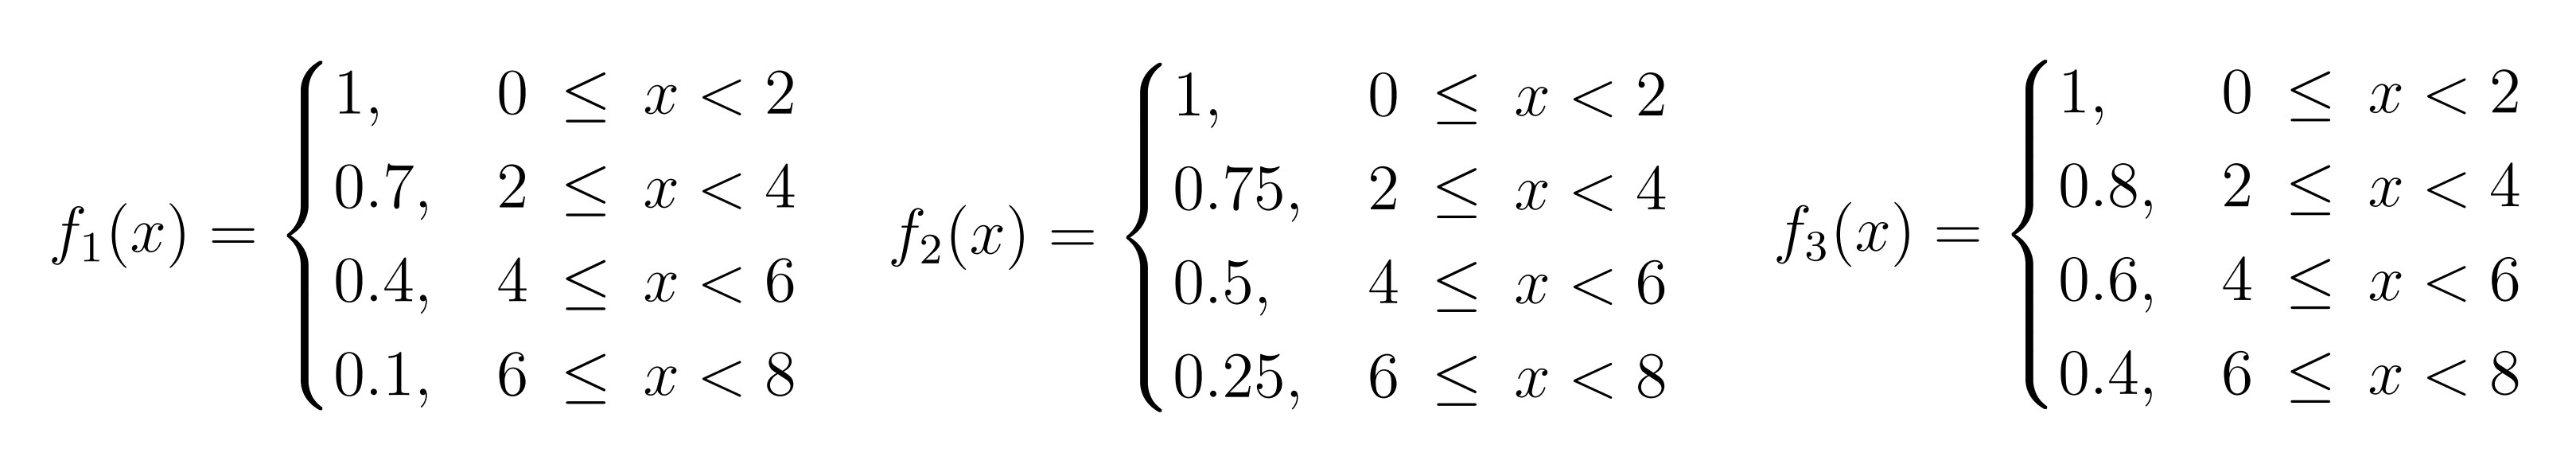
\includegraphics[width=14cm]{gongshi}%图片
\end{figure}


They correspond to three situations with different emphasis on environmental risks. From $ f_{1} $ to $ f_{3} $, people gradually increased the emphasis on risk.


We then built the following predictive function:
\begin{equation}
N_{EDP}(t)=\sum_{i=1}^{countries}\dfrac{\sum_{\delta=1}^{4}f(x)S_{i\delta}(t)}{S_{i}(0)}(1+r_{i})^t
\end{equation}

$\delta$ is the land type.$ S_{i}(0) $is the area of a country at the initial moment.$ S_{i\delta}(t) $is the land area of the country at time $ t $. $ r_{i} $ is the country's population growth rate, taking the average value in the past three years.

Combining the land elevation data we collected, we plotted the predictions on a world map:
\begin{figure}[h]%图片
	\small
	\centering
	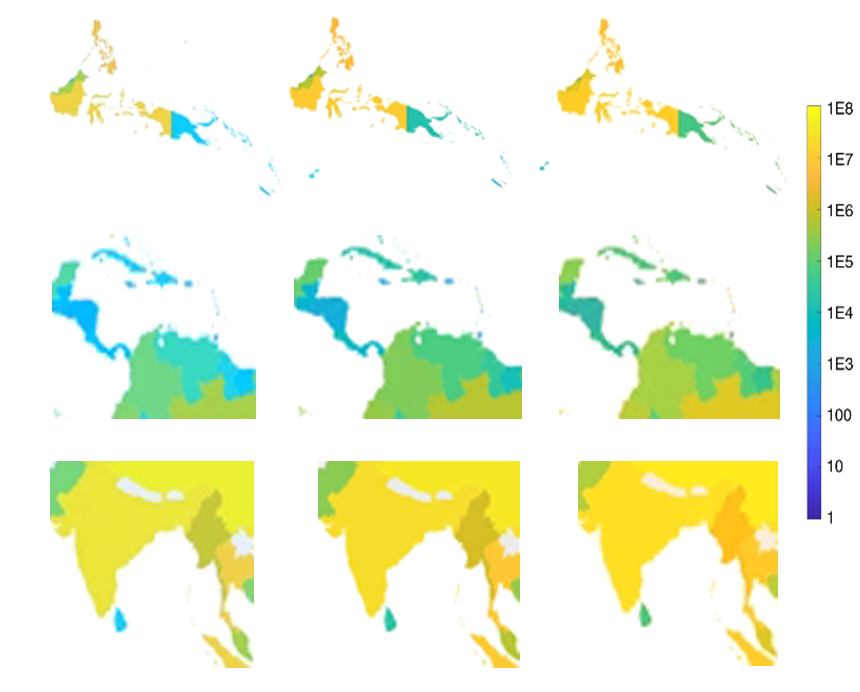
\includegraphics[width=7.5cm]{map}%图片名
	\caption{Sea level height prediction} 
\end{figure}


They are obtained under the conditions of functions$ f_{1}(x),f_{2}(x),f_{3}(x)  $. We chose to use different colors to indicate the number of potential EDPs. Through observation, we can find that the corresponding colors in the three pictures of the same country gradually change from cool to warm, which shows that as the proportional function changes, the number of people who choose to migrate is also increasing. Because this is a result based on the global coastal land elevation data, a large number of people who migrate domestically are also considered.So people who migrate across countries (mainly island nations) are less prominent. But this just shows that we are considerable when making predictions. In the following sections, we will focus on the transnational migration of EDPs in order to meet the main objectives of the United Nations in formulating international policies.































\section{The risk of loss of culture}
\subsection{Risk assessment model for cultural loss}

In this section, we analyze the future of cultural retention after the move of EDPs. The risk assessment model of cultural loss is established by using the gray correlation analysis system (GRA method).

The following assumptions are made to build the model:
\begin{enumerate}
	\item The more similar migration destination culture to the EDPs group culture, the lower risk of cultural loss;
	\item In the light of the actual situation, most of the cultural projects owned by the island countries that become environmental refugees are intangible cultural heritage, and the architectural culture is negligible;
	\item The degree of cultural similarity is related to the following aspects: language culture, religious belief, special customs;
	\item Taking into account that the environment with a large climate difference may not be conducive to the use of the original culture of the EDPs group in life, we also use the latitude difference before and after migration as an influence factor. 
\end{enumerate}

Based on the above assumptions, we assessed the risk of cultural loss after moving to different regions  using the Maldives, Tuvalu, Kiribati, and the Marshall Islands as four representative EDPs origins.  

Based on data from last decade\upcite{2},we identified the countries that received the highest number of refugees worldwide, as shown in the following table:
\begin{figure}[h]%图片
	\small
	\centering
	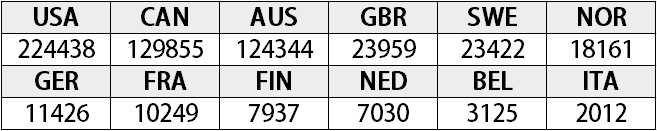
\includegraphics[width=9cm]{jieshouguo}%图片名
\end{figure}

The above data are good references, but given the particularity of EDPs, environmental factors should also be important in the choice of their destination. So based on special considerations of climate and culture, we excluded the countries at high latitudes and included the emerging countries, where the number of immigrants has risen rapidly in recent years, and finalized ten more typical refugee recipient countries. They are: USA, GER ,KSA, RUS, GBR, FRA, UAE, CAN, AUS, ITA. 

Subsequently, we qualitatively measured the cultural indicators of the four EDPs groups and the ten potential major refugee recipient countries, giving them different scores for numerical comparison. 

Where, the cultural reference of the $i^{th}$ EDPs group is marked as$(y_{i}'(1),y_{i}'(2),y_{i}'(3),y_{i}'(4))^T$

The reference to the $j^{th}$ receiving country is marked as$(x_{j}'(1),x_{j}'(2),y_{i}'(3),y_{i}'(4))^T$

Prior to the comparison, we conducted a preliminary examination of the scores of potential refugee recipient countries by means of meanization. The formula is as follows:
\begin{equation}%公式
x_{i}(k)=\dfrac{x_{i}'(k)}{\frac{1}{10}\sum_{i=1}^{10}x_{i}'(k)},k=1,2,3,4 
\end{equation}

We use the cultural indicator of the EDPs as the reference state, and the indicator of the potential recipient country as the actual state, defining the coefficient $ \xi_{ij} $.It represents the relationship between the comparison vector$ x $ and the reference vector$ y $.  In particular, 
\begin{equation}
\xi_{ik}=\dfrac{\min\limits_i\min\limits_k\vert{y(k)-x_{i}(k)}\vert+\rho\max\limits_i\max\limits_k\vert{y(k)-x_{i}(k)}\vert}{{\vert}y(k)-x_{i}(k)\vert+\rho\max\limits_i\max\limits_k\vert{y(k)-x_{i}(k)}\vert}
\end{equation}

Let the association factor $\rho=0.5$ which is the most common value of $\rho$.The degree of association can be given as
\begin{equation}
r_{i}=\frac{1}{4}\sum_{k=1}^{4}\xi_{i}(k)
\end{equation}

After the visualization processing,we can get the chart below:
\begin{figure}[h]%图片
	\small
	\centering
	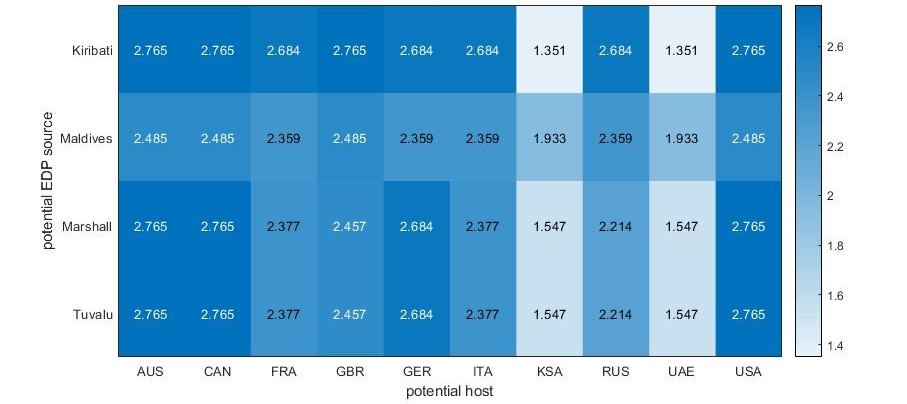
\includegraphics[width=14cm]{gprheatmap}%图片名
	\caption{The risk assessment of cultural loss}\label{fig:7}%题注
\end{figure}

By using this correlation coefficient, the UN can measure cultural differences between receiving countries and EDPs in order to minimize the risk of cultural loss by selecting culturally similar countries as receiving countries.



\subsection{Cultural communication model based on cellular automata}
In order to simulate the collision and integration between the culture of the EDPs and receiving country in the process of cultural exchange, we make the following assumptions:
\begin{enumerate}
\item Only individuals who have grown up to a certain age will participate in the process of cultural exchange. For example, babies and elderly people will not participate in cultural exchanges. Every individual involved in the exchange is equally active.
\item At the beginning of immigration, all individuals have the same degree of inclination to the local culture.Then, the degree of inclination to the two cultures is influenced by the people around him.
\item The age structure of the population of the receiving country and EDPs does not change over time -- this means that the number of individuals involved in the process of cultural exchange does not change.
\item The children's cultural inclination is determined by their parents' .
\end{enumerate}


In the simulation process, we first used a 100$*$100 cell group to simulate the living environment of local residents and EDPs after immigration. Each non-empty cell represented an individual , with a value range of (-1,1). The greater the absolute value of the cell , the more catagorical the individual's inclination. At the beginning, the EDP's inclination toward the receiving country's culture was -1, and the residents' inclination toward their own culture was 1. The entire array can be called a "state", which is used to indicate the position of each individual at this time and the degree of inclination for the two cultures. Subsequently, we chose a month as the status update cycle based on the reality.

When the status is updated, the positions and values of all individuals change simultaneously.

For the change of position, we make the following explanation: Generally, according to the position of the cell in the array, there are 3-8 unequal surrounding cells, which represent other individuals who frequently contact this individual. This is shown in Figure \ref{yuanbao}(a) and Figure \ref{yuanbao}(b) below. Noted that "surrounding" here does not refer to people within a certain distance around the individual, such as people in front of the queue, but refers to people who frequently culturally communicate with the individual during the two updates, such as someone's net friends and penpals. With each update, the cell selects an empty cell around it according to the probability, and exchanges the position with it. The selection probability is shown in the following Figure \ref{yuanbao}(c).
\begin{figure}[H]%并列图片
	\centering
	\subfigure[1]{
	\begin{minipage}{3cm}
		\centering
		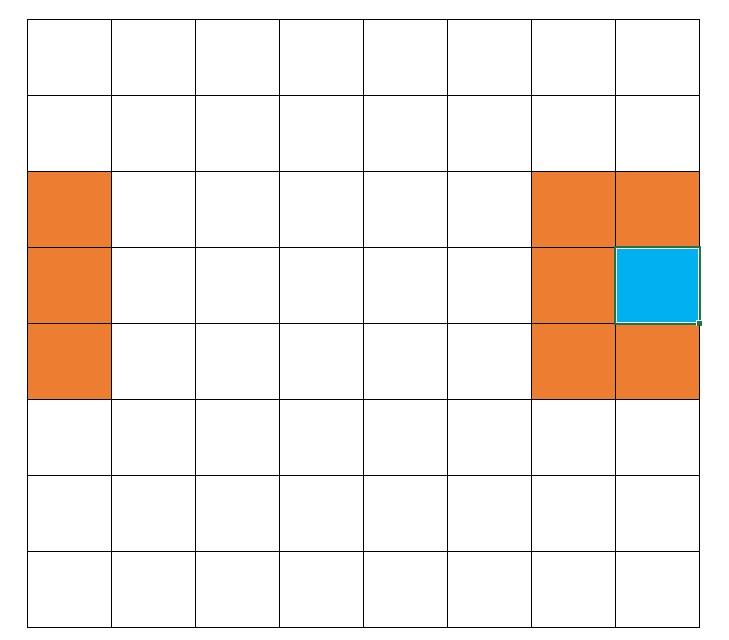
\includegraphics[scale=0.153]{yuan1}
	\end{minipage}
}
\subfigure[2]{
	\begin{minipage}{3cm}
		\centering
		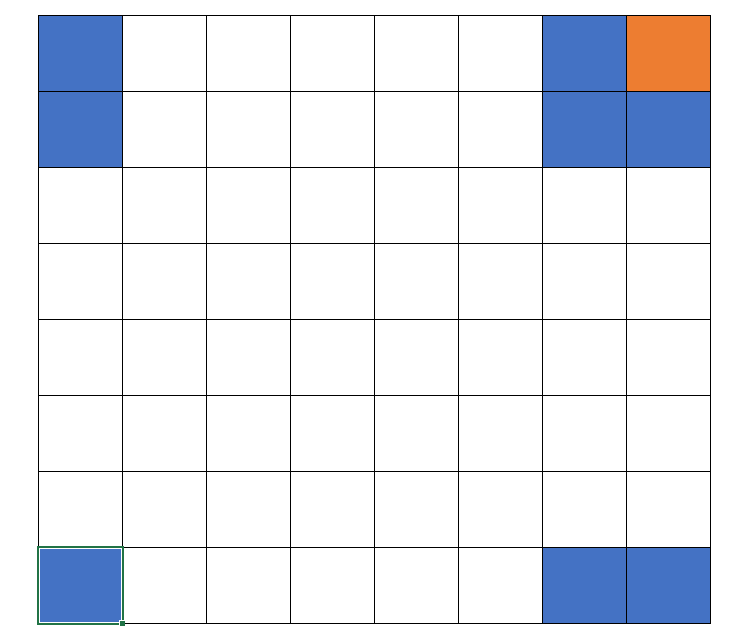
\includegraphics[scale=0.153]{yuan2}
	\end{minipage}
}
\subfigure[3]{
	\begin{minipage}{3cm}
		\centering
		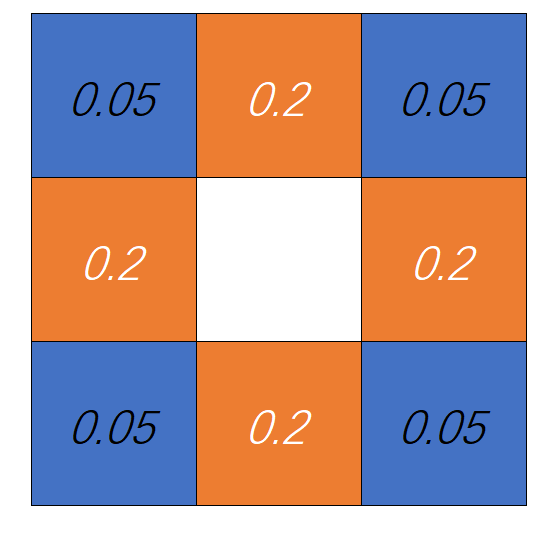
\includegraphics[scale=0.19]{yuan3}
	\end{minipage}
}
\subfigure[4]{
	\begin{minipage}{3cm}
		\centering
		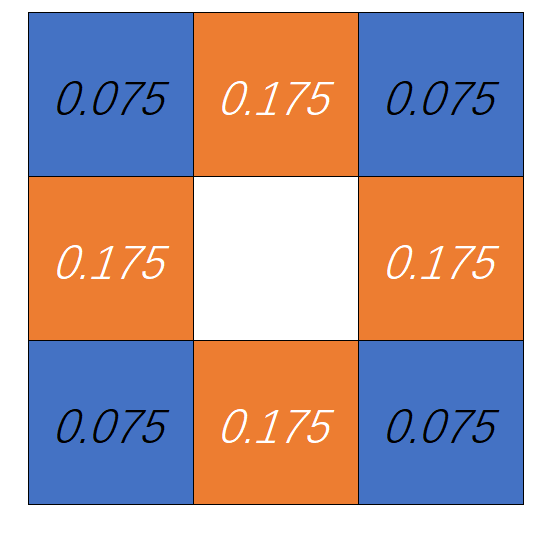
\includegraphics[scale=0.19]{yuan4}
	\end{minipage}
}
\caption{cellular automata}\label{yuanbao}
\end{figure}


For numerical changes, we make the following explanation: the degree of each individual's inclination to two cultures is affected by people around him. During each state update, the value of each cell is changed by the values of its surrounding cells and its own value. That is,
\begin{equation}
	cell_{new}=f(cell_{now} , cell_{surround})
\end{equation}
Where, $ cell_{surround} $ is the weighted sum of the surrounding cell values. Because in reality, people are affected to varying degrees by surrounding individuals, it is reasonable to set different weighted values for surrounding cells. Figure \ref{yuanbao}(d) shows the weighted value we set.

At the same time, we consider that people in different cultures have different levels of difficulty in receiving other cultures, which mainly depends on the actual cultural differences between the two places. We used the GRA value obtained before and made some modifications:
\begin{equation}
	GDA'=min\{-ln(\dfrac{GRA}{max\{GRA\}}),0.05\}
\end{equation}

 The above changes can be expressed as:
\begin{equation}
f(cell_{now},cell_{surround})=arctan(\dfrac{cell_{now}+cell_{surround}{\times}GRA'}{1+GRA'}){\times}\frac{4}{\pi}
\end{equation}

Using the above formula, we simulate the process of cultural exchange, and get the following fusion status in different periods:

\begin{figure}[h]%三因子
	\small
	\centering
	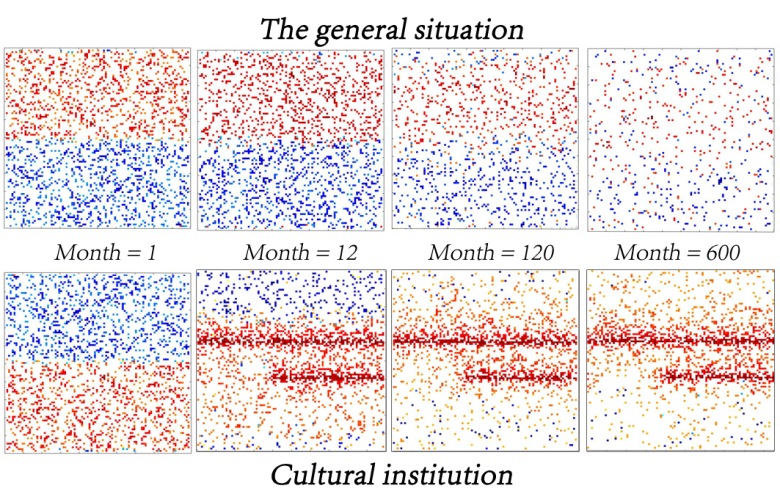
\includegraphics[width=12cm]{diandian}%图片名
	\caption{Fusion status in different periods}
\end{figure}

Subsequently, as a factor closely related to cultural transmission, we added the role of cultural institutions in this process. Cultural institutions are represented by a series of cells with absolute values of 1 in the cell array, which in reality include but are not limited to churches, cultural squares and schools. We assume that once a cultural institution is established, it will not disappear and every individual around it will be edified. Again, we draw scatter charts to show the cultural integration as above.

Through comparison, we can easily find that the function of cultural institutions is to make different cultures solid territories. However, in combination with the images, the receiving country’s culture is often stick to the end. In reality, the local culture often assimilates or absorbs the culture of EDPs group because of fighting on their own soil. However, it also reminds us that EDP cultural institutions can be established to enhance their ability to maintain their own characteristics.

\section{Proposal of policies} 
\subsection{Measuring the benefits and cost}

In this section, we measured the impact of receiving EDPs from the perspective of receiving countries, and explored the internal reasons for whether to take the EDPs or not. We divided the impact of accepting EDPs into benefits and costs, which can be seen as the two sides of a coin. 

From the benefit perspective, receiving EDPs can bring relatively inexpensive labour resources to the receiving country, complement the cultural diversity of the receiving country, and ultimately enhance the receiving country's international reputation and influence. From the cost perspective, receiving EDPs will inevitably squeeze the per capita land area and job opportunities of the local residents, while negatively affecting the country's per capita GDP. The residents' will about receiving EDPs should also be taken into account.We have reasons to believe that when the discontent of residents reaches a certain level, it will lead to social unrest. 

We consider the benefits of taking in EDPs first.Benefit$ (B) $ is used to represent the gross benefit, which can be expressed as the sum of labor resources$ (L) $,cultural diversity$ (Cd) $,and international reputation$ (Ir) $. Assuming that the total number of EDPs received by a receiving country is $ x $. The above three receipts are ,obviously very reasonable, in relation to $ x $ .For example, more migrants would bring more labour to the receiving countries.And the more EDPs groups inflow into a receive country,the more multiple culture will be. So here gives the formula:
\begin{equation}
B(x)=L(x)+Cd(x)+Ir(x)
\end{equation}

After the preliminary analysis, it is not difficult to conclude that $ L(x),Cd(x),Ir(x) $ are all positively related to $ x $ .If it is under the additional assumption that the age structure of the refugee is  basically the same, we can further determine that the relationship $ L(x) $ with $ x $ is linear. That is, $  L(x)=k_{1}x $ ,$ k $ is a proportional factor related to the age structure.  However, the exact relationship $ Cd(x),Ir(x) $ with $ x $ is largely influenced by specific factors such as the size of  receiving country, the origin of EDPs and other factors. Mathematical parsing may have many possible forms. Here we only give a reasonable hypothesis. 

In terms of $Cd(x)$, we will inevitably quantify the unique culture that is contained in an EDP group itself. As we made in section 2.3, the risk assessment model for cultural loss, we can divide the culture of an EDPs group into several or even tens of different dimensions, each of which is calculated as a standard unit of culture. 
Assuming that the cultures in each EDPs group are different, and after repeatedly measuring the importance of all aspects of culture, we have modified and expanded the cultural scope of the previous assumptions to the following form:
$ Culture = \{ language, faith, architecture, songs \& dances, literature, customs, festival \} $
Cultures in each EDPs group can be divided into these seven areas. Because cultures vary from group to group, the increase in cultural diversity after receiving a EDPs group can be simply represented as the sum of the amount of culture brought from each EDPs group. Naturally, we introduce the following formula:
\begin{equation}
Cd(x)=\sum_{i=1}^{m}C_{i}f(x_{i}),s.t.x=\sum_{i=1}^{m}x_{i}
\end{equation}

where $m$ is the number of EDPs groups migrating to the country, $f(x_{i})$ is a function of the number of EDPs$ (x_{i}) $.  Taken the reality into account, it is clear that 1,000 refugees from the same country carry no more than 100 more cultures than 100 refugees from that country.  So we assume that  $f$  is positively correlated with $x$, but the growth rate is gradually slowing down. 

Without loss of generality, let $ f(x_{i})=k_{2}ln(x_i+1) $. 

The amount of culture $ C_{i} $ represents the proportion of unique culture satinted in the cultural dimension of the $ i^{th} $ EDPs group. Therefore, C can be demonstrated as:
\begin{equation}
C=\dfrac{kinds\ of\ culture\ brought}{7}
\end{equation}

Finally, consider $ Ir(x) $. We use some knowledge of microeconomics to treat the reception of refugees as a unique productive input , the benefits of international reputation and international influence as corresponding output. According to the firm's theory, $ Ir(x) $ should have the property of diminishing marginal utility. It is also reasonable to put it in practice : When a country accepts foreign migrants , people will praise its sense of responsibility .But it seems that , in terms of international status, there won't be a significant difference between accepting a large number and a very limited number of migrants , unless some countries use it as a tool to attack others . So we can apply function f to this with just a little change:
\begin{equation}
Ir(x)=k_{3}ln(x+1)
\end{equation}

Here, we come up with a more specific expression of the benefits of receiving imagrants.
\begin{equation}
B(x)=L(x)+Cd(x)+Ir(x)=k_{1}x+\sum_{i=1}^{m}{C_{i}k_{2}ln(x_{i}+1)+k_{3}ln(x+1)}
\end{equation}

Then consider the measure of the cost of accepting migrants.

We use Expenditure (E) to represent the total cost, then it can be expressed as the sum of area cost (S), per capita GDP cost (G), and social unrest cost (Su). To simplify the model, it can be assumed that the EDP will not be able to generate significant GDP for the receiving country within a period of time after the migration. And the receiving country often has such a trend: the EDPs are placed in a region with a small population density. So the per capita area occupied by the local residents is not greatly affected. The area cost is only the potential value of land allocated for the EDPs. We can simply think that the area of land is proportional to the number of EDPs.

The total area of the receiving country j is $ S_{j} $ , the total GDP is $ {GDP}_{j}$ , the total population is $ N_{j} $ , the number of migrants admitted is $ x $ ,then
\begin{equation}
S_{j}(x)=l_{1}x
\end{equation}
\begin{equation}
G_{j}(x)=\dfrac{l_{2j}GDP_{j}x}{N_{j}(N_{j}+x)}
\end{equation}

Measure of the cost of social unrest $ Su(x) $ is more complex.The possibility of social unrest is influenced by the residents' ideology of the receiving country and the national openness degree. The greater cultural differences between EDPs and the residents of the receiving country are, the more likely cultural conflicts happen. We even do not rule out that the issue of migrants has become a powerful tool for campaigning between different political parties. 

For example, social contradictions in a major Nordic refugee-receiving country has been increasing in recent years, largely because of the differences in ideology and religious beliefs between the refugees and local residents. Although the receiving country has adopted a policy of multiculturalism to encourage the development of cultural and religious diversity, it has ,to some extent, contributed to the closure and consolidation of different cultural groups. Instead of integrating into mainstream society, the refugees have gradually developed a flat society isolated from mainstream society. This has led to refugees' recognition of the new country far less than the recognition of religious beliefs, and the rejection of refugees by the inhabitants of the receiving countries has gradually increased, resulting in continuation of friction. This is clearly what we don't want to see. 

Based on the above facts, we further divide the cost of social unrest $ Su(x) $ into two parts: resettlement costs $ R(x) $ and security costs $ P(x) $.  Resettlement cost is the human and material which consumed in dividing a certain area of the receiving country's territory and settling EDPs into this area .Security costs is the daily expense to ensure basic social stability after receiving refugees which takes into account cultural conflicts and the scale of influx. 

Under the additional assumption that the number of migrants receiving is much smaller than the number of local residents in the receiving country, we can suppose that the residential areas needed to be divided for EDPs are approximately proportional to the number of EDP people, while the resettlement costs for each unit of land remain unchanged. So we can simply consider that Rx satisfies the following relation formula: 
\begin{equation}
R_{j}(x)=l_{3j}x
\end{equation}
Where, $ l_{3} $ is a constant related to unit placement costs. 

In addition, we combined reality conditions and draw the conclusion: greater cultural differences and larger number of EDPs both make it more difficult for society to maintain stability. At the same time, we find that the number of EDPs is often not linear with the unease level among receiving nations. It may be considered that this uneasiness is a disease that spreads rapidly among the population, and its intensity can be used as a preliminary fit using an infectious disease model. 

Based on the above considerations, we propose the following expression as the security cost incurred by EDPs in the receiving country $j$ :
\begin{equation}
P_{j}(x)=\sum_{i=1}^{m}l_{4j}e^{x_{i}GRA_{ij}}
\end{equation}

$ m $ is the number of EDPs group.$ {GRA}_{ij}$ is a gray correlation analysis indicator derived from the cultural loss risk assessment model.

So far, we've got an expression of the cost of receiving EDPs:
\begin{equation}
E_{j}(x)=S_{j}(x)+G_{j}(x)+Su_{j}(x)=l_{1}x+\dfrac{l_{2j}GDP_{j}x}{N_{j}(N_{j}+x)}+l_{3j}x+\sum_{i=1}^{m}l_{4j}e^{x_{i}GRA_{ij}}
\end{equation}

Overall, each receiving country has a process of measuring the pros and cons before receiving EDPs.Iff $ B_{j}(x)>E_{j}(x) $, country $ j $, as a potential receiving country, will temporarily resettle EDPs on their territory. The UN, as the constitutor of international conventions and policies, can influence EDPs reception activities by adjusting this inequality. Therefore, the analysis of this part has laid a solid foundation to make our own policy proposals to the UN, and we have taken a small step closer to harmonious development of the world. 

\subsection{Policy considerations for the reception of EDPs}

In this section, we will analyse possible policies for the UN from two main perspectives: 

With the principles of fairness and impartiality, the UN should formulate policies based on the root causes of EDPs. Considering the nations' disproportionate contribution to the green-house gasses,they should be mandatorily rule to take EDPs in proportion. Similarly,the nations, which reduced the green-house gasses' emissions,  could reduce the number of EDPs taken .

We consider this question in accordance with the above principles. The world today is facing the problem of global climate change and sea level rise, which is largely the cumulative consequence of the green-house gasses emissions from industrialization. Therefore, it is reasonable to believe that countries with large emissions should assume more responsibilities and obligations for the migration of EDPs. However, some countries have weakened their responsibilities and are reluctant to provide assistance to the EDPs. This makes it difficult for the UN, as a global policy maker, to implement policies and principles in all countries.

\subsubsection{Nations' contribution to the green-house gasses} 

\quad\enspace In the following analysis, we continue to focus on the ten countries which have received most refugees. Most of them are developed countries, but also a few are developing countries. We just take them as a basis for larger-scale research in the future. 

We collect national carbon emission data\upcite{4} and GDP data\upcite{6} for the past decades. A simple indicator $ k_j=\frac{{GDP}_{j}}{{Emission}_{j}} $ can be defined to represent the increase in GDP for each unit of greenhouse gases emitted. The higher the K value is, the more environment-friendly the country's production methods are. Our computing result is shown in Figure\ref{wenshi1}: 
\begin{figure}[H]%温室气体并列图片
	\begin{minipage}[t]{0.5\textwidth}
		\centering
		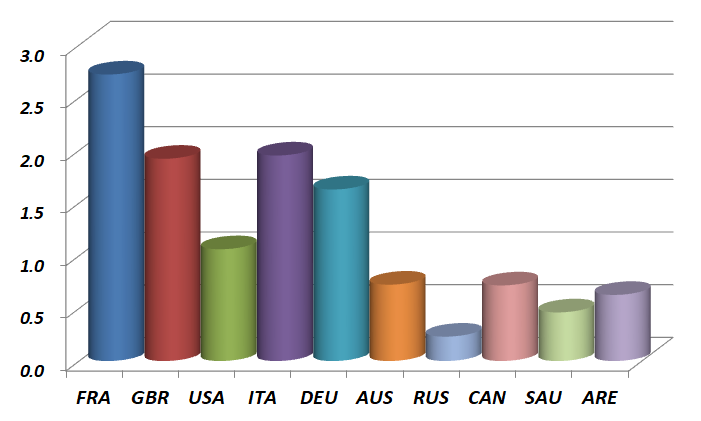
\includegraphics[scale=0.35]{wenshi1}
		\caption{Value of index $ k_{j} $\label{wenshi1}}
	\end{minipage}
	\qquad
	\begin{minipage}[t]{0.5\textwidth}
		\centering
		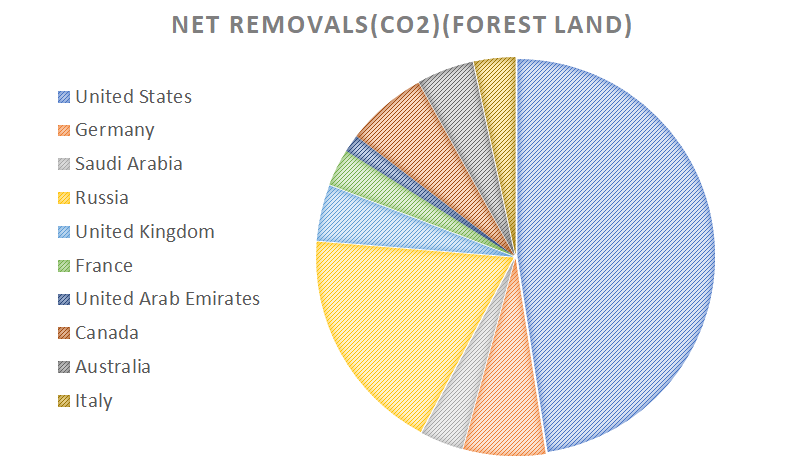
\includegraphics[scale=0.32]{wenshi2}
		\caption{Forest carbon absorption\label{wenshi2}}
	\end{minipage}
\end{figure}

Moreover, we investigate the carbon absorption in these countries. Natural green vegetation is the main force for carbon absorption. After reviewing biological data, we find that the carbon absorption capacity of forests and grasslands is quite different. The carbon storage of tropical savannas is less than 1/10 of the forest, and there is even two orders of magnitude difference between the carbon sequestration capacity of temperate grasslands and forest. So it is logical to ignore the carbon sequestration of grasslands when calculating carbon absorption, and only consider that of the forest. According to the data after 2000,we calculated the proportion of forest carbon absorption of these countries , given as $ {rem}_{j} $, j=1,2,...,10, as shown in Figure \ref{wenshi2}.  	

We combine the two parameters above as a reference to determine the amount of EDPs that are forced received. Formula \eqref{kj} is a common type of excitation function in the neural network to normalize the k value.
\begin{equation}%公式
f(k_{j})=\dfrac{1-e^{-k_{j}}}{1+e^{-k_{j}}} \label{kj}
\end{equation}

Then, by calculating the arithmetic mean of \ $ f(k_{j}) $ and $ {rem}_{j} $ ,we get a relatively comprehensive index. 
\begin{equation}%公式
El_{j}=\frac{1}{2}(f(k_{j})+rem_{j})
\end{equation}

A larger value of $ {El}_{j} $ means that the country's production methods is more environment- friendly and has less influence to the sea level rise. In reality, the above indicators to a certain extent to explain the actual situation. For example, France vigorously builds nuclear power. It's carbon emission reduction results are excellent in the world, so the environmental protection index is reasonable to become the highest of the ten countries. Saudi Arabia and the United Arab Emirates, as desert countries, have less green space and less carbon-absorbing contributions, which are ultimately reflected in a lower environmental index. 

\subsubsection{The ratio of compulsory acceptance}
%强制人数

\quad\enspace By using the environmental protection index, per capita GDP, and land area as the influential factors, we formulated the compulsory acceptance ratio, analyzing with the analytic hierarchy process (AHP). The main step of AHP is to compare the status of different influencing factors and store them in the weight matrix, and then substitute them into each scheme and calculate the corresponding eigenvalues. Here, we use ten major refugee-receiving countries as alternatives to calculate the score of their reception portion.

We created a weighting matrix of three importance factors based on the following considerations:

Economic capacity (reflected in per capita GDP) is obviously the first factor to measure a country's ability to objectively accept EDPs without being affected, so we have appropriately increased its importance in the weight matrix. Additionally, land area is the most intuitive indicator representing the size of the receiving country. However, in reality, a country with a large land area may not necessarily have strong comprehensive strength. This is due to the restriction of land types. So we include it in the measurement system, but not giving too much weight. Finally, we include the environmental index just calculated. As an encouragement to the environmental protection career of some countries, the environmental protection index will be negatively related to the compulsory acceptance ratio, so we made a change of it's form :
\begin{equation}
EI_{j}=1-\dfrac{EI'_{j}}{max\{EI'_{j}\}}
\end{equation}

The weight matrix is as follows:
\[W^{(2)}=
\begin{pmatrix}
{1} & {4} & {2}  \\
{1/4} & {1} & {1}  \\
{1/2} & {1} & {1}  \\
\end{pmatrix}
\]

Where, factor 1 is the per capita GDP, factor 2 is the land area, and factor 3 is the environmental protection index.

The weight matrix is inconsistent, so it is necessary to check whether the degree of inconsistency meets the requirements of the AHP method:

\begin{equation}
	CI=\dfrac{\lambda_{max}-3}{2}=0.0268
\end{equation}

Then, the consistency ratio is

\begin{equation}
CR=\frac{CI}{RI}=0.0462<0.1
\end{equation}

Therefore, it can be considered that the error is within the allowable range. Normalize the corresponding eigenvector of $\lambda_{max}$ .The result is:
\begin{equation}
\overrightarrow{w}^{(2)}=(0.5842, 0.1840, 0.2318)
\end{equation}

Subsequently, we normalize the per capita GDP and land area of each country ,and form a table with the processed EI index:

\begin{figure}[h]%三因子
	\small
	\centering
	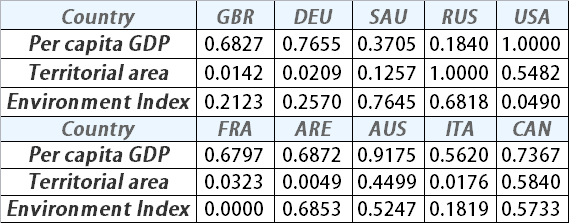
\includegraphics[width=10cm]{sanyinzi}%图片名
	\caption{Value of the EI index}
\end{figure}

Combining the above two indicators with the processed environmental protection index, we use the same method to construct a pairwise comparison matrix of influencing factors in each receiving country. Then we calculate the normalized eigenvector corresponding to the maximum eigenvalue of each comparison matrix, and combine them as column vectors to form a matrix:
\begin{equation}
	W^{(3)}=(w_{1},w_{2},w_{3})
\end{equation}

The combined weight vector of each receiving country to the target layer is
\begin{equation}
\overrightarrow{w}^{(3)}=W^{(3)}\overrightarrow{w}^{2}
\end{equation}


\begin{figure}[h]%比例
	\small
	\centering
	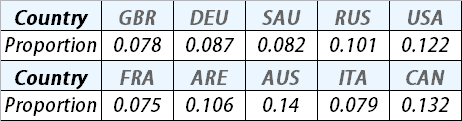
\includegraphics[width=8cm]{ratio}%图片名
	\caption{The ratio of compulsory acceptance} \label{fig:ratio}%题注
\end{figure}

Figure \ref{fig:ratio} shows the percentages of mandatory reception that the ten major refugee receiving countries shoule be responsible for.
%补充


Based on the above analysis and distance between countries,we gave a rational migration path plan.The result is in Appendix C.




\subsubsection{A game theory model of EDPs and receiving country}
\quad\enspace On the basis of the mandatory receiving provision , we take into account the actual situation. Some of the assumptions in the previous statement are added and amended as follows:
\begin{enumerate}
\item EDPs are fundamentally different from other refugees, after moving to the receiving country, they should have the right to choose freely whether to maintain their original lives on the new land without having more contact with the local residents and society , or  gradually assimilate into the new social environment and embrace the new culture. 

\item When EDPs make decisions to maintain their original lives, they have no benefits or costs. When EDPs make decisions to assimilate into the new society, they earn more than they did in their original lives, but may lose their culture and be discriminated against by local residents. 

\item When EDPs make the decision to maintain the original life, the receiving country receives the international reputation benefit, which requires the land area cost, the resettlement cost. When EDPs make the decision to integrate into the new society, the receiving country receives the benefits of labor, cultural diversity, and international reputation, but also pays the land area cost,GDP cost, placement cost and security cost. 

\item When EDPs want to integrate into a new society, the host country of the refugee can accept them or refuse to accept them privately. But refusal to accept is an act that is inconsistent with the provisions of the UN and has the potential to be detected by the UN and punished accordingly. 
\end{enumerate}

Based on the above assumptions, we conclude that another aspect of United Nations policy development is the punishment of receiving countries that do superficial articles.
The parameters used in this section are described below: 
\begin{table}[h]%符号
	\begin{tabular}{ll}
		\hline
		Notions           & Description                                                                                                                                    \\ \hline
		$w$               & Total net growth of EDPs' income after assimilation                                                                                          \\
		$P_{1}(GRA_{ij})$ & The probability of cultural loss and suffering discrimination after assimilation.                                                              \\
		$a_{1}$           & The loss of EDPs due to cultural loss and discrimination.                                                                                      \\
		$P_{2}$           & \begin{tabular}[c]{@{}l@{}}Probability of being found and punished by the UN when the receiving \\ country does superficial work.\end{tabular} \\
		$a_{2}$           & Fines collected by the UN when receiving country violate policy.                                                                               \\ \hline
	\end{tabular}
\end{table}

The above behavior constitutes a game process, we can draw the game's decision tree as Figure\ref{fig:shu}.

\begin{figure}[h]%决策树
\small
\centering
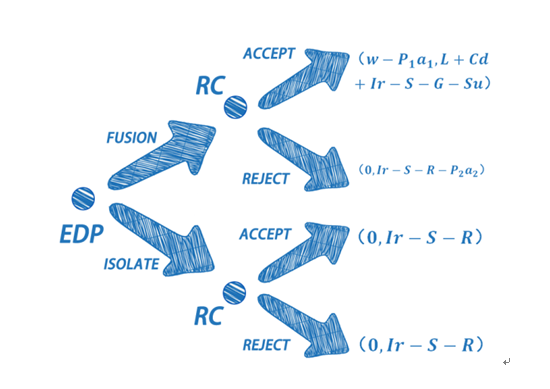
\includegraphics[width=8cm]{jueceshu}%图片名
\caption{Decision tree} \label{fig:shu}%题注
\end{figure}

In the first phase of the game, we consider the decision stake of EDPs. Assuming that both the EDPs and the government leaders of the receiving country are rational people in the economic sense, making decisions by judging the expected benefits. Thus, only when the wealth gains from assimilation outweigh the potential cultural loss and discrimination $ (w-P_{1}a_{1}>0) $, the EDPs choose to integrate into the new society. Otherwise they will maintain a relatively closed life.
 
Following EDPs, the receiving country will also make a decision. 

When EDPs choose to maintain its original lifestyle, the decision of receiving country will have no effect on the outcome of the game.When EDPs choose to integrate into the new society, the situation becomes a bit complicated. The receiving country can either follow the choice of the EDPs or refuse their request at the risk of being punished by the UN. It is easy to note that this depends on the net income difference between two options. Only when$  L+Cd+P_{2}a_{2}-G-P>0 $ ,the benefits of taking EDPs outweigh the risks incurred when rejecting. Under this circumstance ,the receiving country may choose to take the EDPs and become a real family with them as time goes on.

According to the purposes of the UN, we know that its mission is to achieve, as far as possible, a win-win balance. The UN should consider both the gains of receiving country and the interests of the EDPs. 

Through $  P_{2}a_2>G+PL-L-Cd $ , it can be found that, the UN should strengthen the supervision of the receiving countries  , increasing $ P_{2} $, so that some violations of the provisions have nowhere to hide . Also it should moderately raise fines$ a_{2} $ , in order to achieve effective deterrence. 

%新增

Next we consider the subjective initiative of the EDPs and the receiving country. When the EDPs are reluctant to integrate into the new society, but its integration can bring considerable dividends to the receiving country, that is
\begin{equation}
\begin{cases} w-P_{1}a_{1}<0,\\
L+Cd-G-P>0,
\end{cases}\label{kuohao}
\end{equation}

When (\ref{kuohao}) is true, the receiving country can impel the EDPs to change its choice by transferring a portion of the profit to the EDPs. Such measures include, but not limited to, improving treatment of EDPs in new jobs and promoting cultural acceptance around the country's residents. As long as the sum of the benefits of then is satisfied $ L+Cd+w-P-G-P_{1}a_{1}>0 $ there is a possibility that EDPs will change the decision. 

Such measures are easy to think of and accept, meanwhile, consisting with the goal of the UN to maximize the sum of the benefits. But it also has potential problem. We consider that the strength of EDPs community is too small compared to the major receiving countries. This may lead to several major receiving countries reducing the benefits of EDPs  through setting up alliances.  "Since the EDP group is rational, the recipient country will choose to integrate into the new society as long as it ensures that the benefits ofEDP after entering the new society are slightly higher or even equivalent to the benefits of the closed   society." The end result is that the major refugee-receiving countries enjoy the dividends of the labour force brought to them by the arrival of refugees, but are obediated about the state of life of the EDP group itself. This is clearly not in line with our intention. 
In this case, we can solve this by calculating the following factors:
\begin{equation}
	alpha_{ij}=\dfrac{\frac{1}{x_{i}}(w-P_{1}a_{1})}{\frac{1}{N_{j}}(L+Cd-G-P)}
\end{equation}

$ \alpha_{ij} $ measures the improvement of life quality of the EDPs group i in receiving country j. If, when distributed equally to the individual, each EDP receives far less benefit than the domestic residents of the receiving country, we can assume that the country's approach is unfair. There is no possibility that $ \alpha_{ij} $ exceeds 1 for a long time due to the wide disparity between the force of EDPs and the receiving country.  Therefore, setting the minimum standard for $ alpha_{ij} $ close to 1 (e.g.0.8) will help to improve EDP life. These improvements can be fed back to the EDPs as a spiritual support for a sense of belonging, which is the embodiment of the policy to protect  human rights.  


\subsection{Policy assessment model}
This model intends to evaluate the risk and the extra costs it brings in aspect of probability.
The basic structure of the Bayesian network is as follows:

\begin{figure}[h]%
	\small
	\centering
	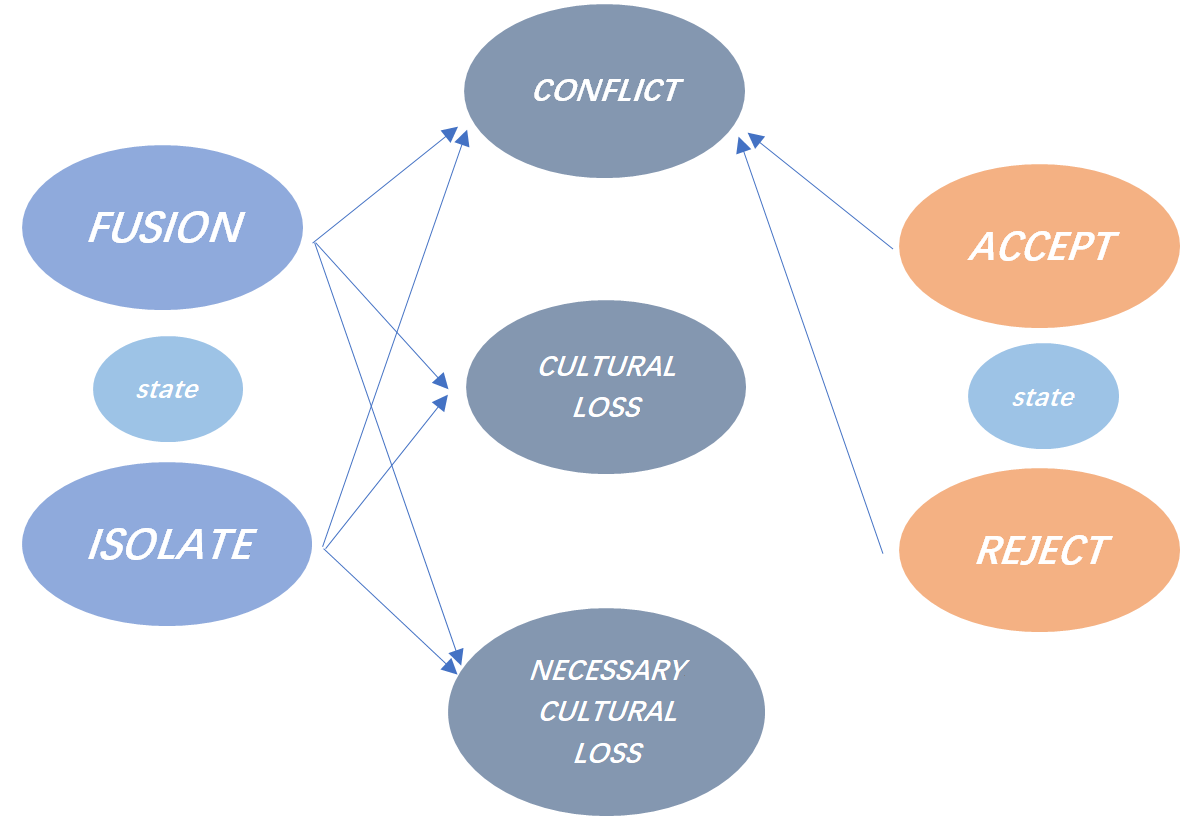
\includegraphics[width=8cm]{by}%图片名
	\caption{Structure of Bayesian network} 
\end{figure}




This model makes the following assumptions:
\begin{enumerate}

\item EDPs are regarded as “fusion” if over eighty percent of them learn the language of R country, believing in local religion (only considered in countries with unification of the state and the church), participating in local traditional festivals, and are regarded as “isolate” if only a minority do so.
\item Receiving countries are regarded as \textbf{accepting} the EDPs if they initiatively afford a portion of the expense in migration, settlement and public security of the refugee, and regarded as \textbf{rejecting} in the opposite situation.
\end{enumerate}

The bottom event of this network is the state of receiving countries (here referred to country R ) and the EDPs, including the cultural difference$ (k) $, the climate difference$ (d_{cd}) $, the population of R country and the EDPs that migrate in $ (P_{r},P_{e}) $, the gross national income $ (GNI) $ and gross domestic product $ (GDP) $ of R country, the cultural diversity $ (Cd) $ of R country, the national territorial area of R country, the estimated expense of migration$  (E_{me}) $, necessary cultural loss $ (l_{nc}) $, reputation loss for rejecting the refugee$ (lr) $, and the net export of R country. 

Most of the elements, including$  k, d_{cd}, P_{r}, P_{e}, GNI, GDP, Cd, $ are either explained previously, the explanations of the rest are as follows:
\begin{figure}[h]%
	\small
	\centering
	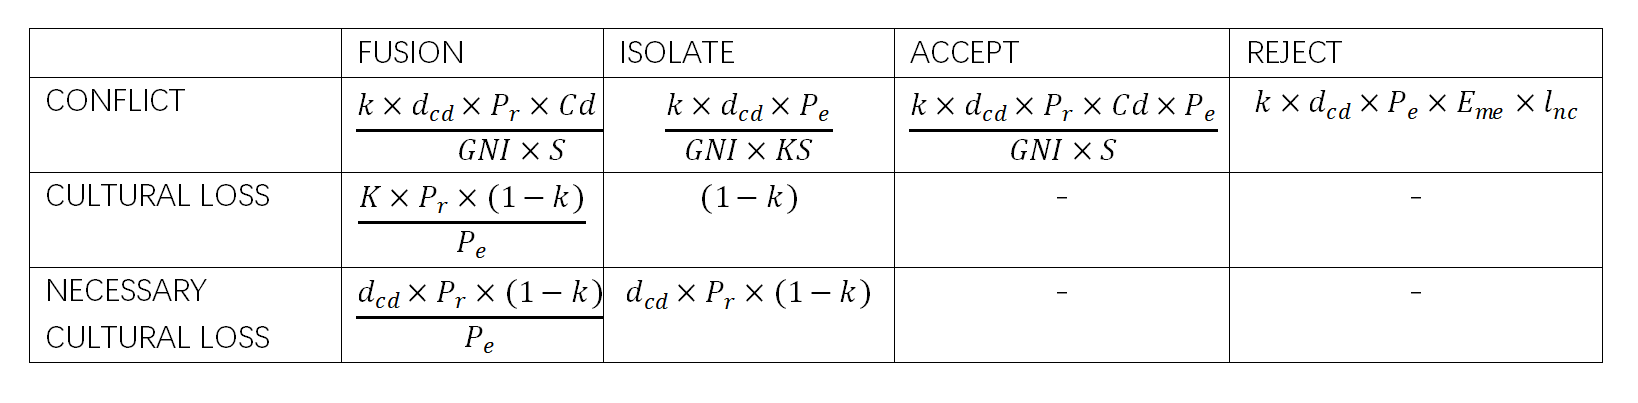
\includegraphics[width=16cm]{biao}%图片名
\end{figure}

The climate difference of two countries relies mainly on its precipitation and average temperature each month, expressed as $ pr_{(i)}, pe_{(i)}, tr(i), te_{(i)} $.Then, $ d_{(cd)} $ can be defined as:

\begin{equation}
d_{cd}=\dfrac{(\sum_{i=1}^{12}(pr_{i}-pe_{i})^{2}+\sum_{i=1}^{12}(tr_{i}-te_{i})^{2})}{2}
\end{equation}

The estimated expense of migration is apparently in proportion to the amount of EDPs and the distance of migration, expressed as:
\begin{equation}
E_{m}=w{\times}P_{EDP}{\times}D_{migration}
\end{equation}

There are two kinds of necessary cultural loss. One is the culture must relies on a entity, such as the Temple Compounds of Sri Lanka. The other one is based on some certain environment, sea fishing for instance. Neither of them will last when environment changes.

The reputation loss for rejecting the EDPs is evaluated by the portion that net export accounts for of GDP. Obviously, countries which relies on national trades will attach more importance to its reputation, and less likely to reject. So the equation can be given is:
\begin{equation}
lr=\frac{ne}{GDP}
\end{equation}

The probability of a top events being affected by transition layer event can be expresses as :
\begin{equation}
K= average(\frac{S_{e}}{Sr})
\end{equation}
For any top events and transition layer events, the contingent probability is 
\begin{equation}
P(top{\vert}transition)=1-e^{x(top,transition)}
\end{equation}
$ x(top,transition) $ refers the index of the table upon,for example:
\begin{equation}
x(CONFLICT{\vert}FUSION)=\dfrac{k{\times}d_{cd}{\times}P_{r}{\times}Cd{\times}lnc}{GNI{\times}S}
\end{equation}





\section{Strengths and weaknesses}
\subsection{Strengths}
We use a concise sequential game theory model to describe the decision-making process and equilibrium among EDP, receiving countries and the UN, which is innovative.

When creating parameters, we considered various factor, which allowed the function to accurately describe the overall situation while retaining certain variability for using in different sub-fields.

We combined analytic hierarchy process, Bayesian network, cellular automata algorithm and other research methods to formulate and evaluate policies, and have achieved satisfactory results. It has considerable reference value.
\subsection{Weaknesses}
In the formulation of some parameters, subjective feelings occupy a more important position.

We cannot test the robustness and sensitivity of the model without sufficient data.

In real life, there are far more EDPs and potential refugee receiving countries than the number studied in this paper. The methods and indicators proposed in this paper can be used as examples of reference value, but whether they have broader applicability still remains to be tested.







\begin{thebibliography}{99}%参考文献
\bibitem{1} Climate.Gov \url{https://www.climate.gov/maps-data}
\bibitem{2}The UN Refugee Agency \url{https://www.unhcr.org/en-us/data.html}
\bibitem{3}CSIOR.au\enspace\url{https://research.csiro.au/slrwavescoast/sea-level/measurements-and-data/sea-level-data/}
\bibitem{4}Food and Agticulture Organization of the United Nation \url{http://www.fao.org/faostat/en/#data/GF}
\bibitem{5}Yang Guangyi, Jiao Xu Dong, Chen Yongjin, Gao Wei, Cui Jiujie, Wang Xinjing,(2016).Analysis of the impact of global change on the South Pacific island of Tuvalu
\bibitem{6}World Bank Open Data
\bibitem{7}Sun Hualing,(2013).Study on the right of climate refugees to migrate
\bibitem{8}Zhou Yimin,(2018).Exploring the Path of International Mechanism to Deal with Migration —— Taking the European Migration Crisis as an Example
\bibitem{9}Richard Black,(2010). Dominic Kniveton, Kerstin Schmidt-Verkerk.Migration and climate change: towards an integrated
\bibitem{10}Scund J Sac Wel/ctre,(1994).A culturally sensitive 
case-management model: 
the experience of Southeast Asian 
refugeks in Washington State, USA
\bibitem{11}Lanphier, Michael,(1983).Refugee resettlement:models in action
\end{thebibliography}

\newpage
\begin{appendices}
\section{self-correlation and partial correlation analysis}
\begin{figure}[H]%并列图片
	\begin{minipage}[t]{0.5\textwidth}
		\centering
		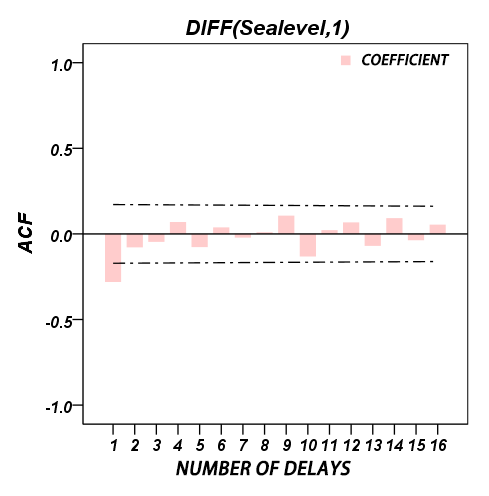
\includegraphics[scale=0.4]{zixiangguanjianyan}
		\caption{Autocorrelation test\label{fig:3}}
	\end{minipage}
	\qquad
	\begin{minipage}[t]{0.5\textwidth}
		\centering
		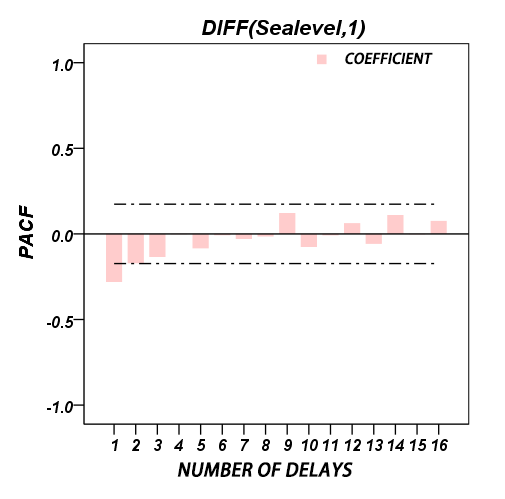
\includegraphics[scale=0.4]{pianzixiangguanjianyan}
		\caption{Partial autocorrelation test\label{fig:4}}
	\end{minipage}
\end{figure}




\section{Matrices of AHP}
\[W_{GDP}=
\begin{pmatrix}
1.00 	&	1.00 	&	2.00 	&	4.00 	&	0.50 	&	1.00 	&	1.00 	&	0.50 	&	1.00 	&	1.00 	\\
1.00 	&	1.00 	&	2.00 	&	4.00 	&	1.00 	&	1.00 	&	1.00 	&	1.00 	&	1.00 	&	1.00 	\\
0.50 	&	0.50 	&	1.00 	&	2.00 	&	0.33 	&	0.50 	&	0.50 	&	0.33 	&	0.50 	&	0.50 	\\
0.25 	&	0.25 	&	0.50 	&	1.00 	&	0.17 	&	0.25 	&	0.25 	&	0.20 	&	0.33 	&	0.25 	\\
2.00 	&	1.00 	&	3.00 	&	6.00 	&	1.00 	&	1.00 	&	1.00 	&	1.00 	&	2.00 	&	1.00 	\\
1.00 	&	1.00 	&	2.00 	&	4.00 	&	1.00 	&	1.00 	&	1.00 	&	1.00 	&	1.00 	&	1.00 	\\
1.00 	&	1.00 	&	2.00 	&	4.00 	&	1.00 	&	1.00 	&	1.00 	&	1.00 	&	1.00 	&	1.00 	\\
2.00 	&	1.00 	&	3.00 	&	5.00 	&	1.00 	&	1.00 	&	1.00 	&	1.00 	&	1.00 	&	1.00 	\\
1.00 	&	1.00 	&	2.00 	&	3.00 	&	0.50 	&	1.00 	&	1.00 	&	1.00 	&	1.00 	&	1.00 	\\
1.00 	&	1.00 	&	2.00 	&	4.00 	&	1.00 	&	1.00 	&	1.00 	&	1.00 	&	1.00 	&	1.00 	\\
\end{pmatrix}
\]

\[W_{s}=
\begin{pmatrix}

1.00 	&	1.00 	&	0.20 	&	0.11 	&	0.13 	&	0.50 	&	2.00 	&	0.13 	&	1.00 	&	0.13 \\
1.00 	&	1.00 	&	0.33 	&	0.13 	&	0.14 	&	1.00 	&	2.00 	&	0.17 	&	1.00 	&	0.14 \\
5.00 	&	3.00 	&	1.00 	&	0.25 	&	0.33 	&	2.00 	&	6.00 	&	0.33 	&	4.00 	&	0.33 \\
9.00 	&	8.00 	&	4.00 	&	1.00 	&	2.00 	&	7.00 	&	9.00 	&	2.00 	&	8.00 	&	2.00 \\
8.00 	&	7.00 	&	3.00 	&	0.50 	&	1.00 	&	6.00 	&	9.00 	&	1.00 	&	7.00 	&	1.00 \\
2.00 	&	1.00 	&	0.50 	&	0.14 	&	0.17 	&	1.00 	&	3.00 	&	0.20 	&	2.00 	&	0.17 \\
0.50 	&	0.50 	&	0.17 	&	0.11 	&	0.11 	&	0.33 	&	1.00 	&	0.11 	&	0.33 	&	0.11 \\
8.00 	&	6.00 	&	3.00 	&	0.50 	&	1.00 	&	5.00 	&	9.00 	&	1.00 	&	7.00 	&	1.00 \\
1.00 	&	1.00 	&	0.25 	&	0.13 	&	0.14 	&	0.50 	&	3.00 	&	0.14 	&	1.00 	&	0.14 \\
8.00 	&	7.00 	&	3.00 	&	0.50 	&	1.00 	&	6.00 	&	9.00 	&	1.00 	&	7.00 	&	1.00 \\
\end{pmatrix}
\]

\[W_{EI}=
\begin{pmatrix}
1.00    &	1.00    &   0.33 	&	0.33 	&	5.00 	&	9.00 	&	0.33 	&	0.50 	&	1.00 	&	0.33 \\
1.00    &   1.00    &   0.33 	&	0.33 	&	6.00 	&	9.00 	&	0.33 	&	0.50 	&	1.00 	&	0.50 \\
3.00    &   3.00    &   1.00 	&	1.00 	&	8.00 	&	9.00 	&	1.00 	&	1.00 	&	4.00 	&	1.00 \\
3.00    &   3.00    &   1.00 	&	1.00 	&	8.00 	&	9.00 	&	1.00 	&	1.00 	&	4.00 	&	1.00 \\
0.20    &   0.17    &   0.13 	&	0.13 	&	1.00 	&	9.00 	&	0.13 	&	0.14 	&	0.20 	&	0.14 \\
0.11    &   0.11    &   0.11 	&	0.11 	&	0.11 	&	1.00 	&	0.11 	&	0.11 	&	0.11 	&	0.11 \\
3.00    &   3.00    &   1.00 	&	1.00 	&	8.00 	&	9.00 	&	1.00 	&	1.00 	&	4.00 	&	1.00 \\
2.00    &   2.00    &   1.00 	&	1.00 	&	7.00 	&	9.00 	&	1.00 	&	1.00 	&	3.00 	&	1.00 \\
1.00    &   1.00    &   0.25 	&	0.25 	&	5.00 	&	9.00 	&	0.25 	&	0.33 	&	1.00 	&	0.33 \\
3.00    &   2.00    &   1.00 	&	1.00 	&	7.00 	&	9.00 	&	1.00 	&	1.00 	&	3.00 	&	1.00 \\

\end{pmatrix}
\]


\section{A rational migration path plan}
\begin{figure}[h]%
	\small
	\centering
	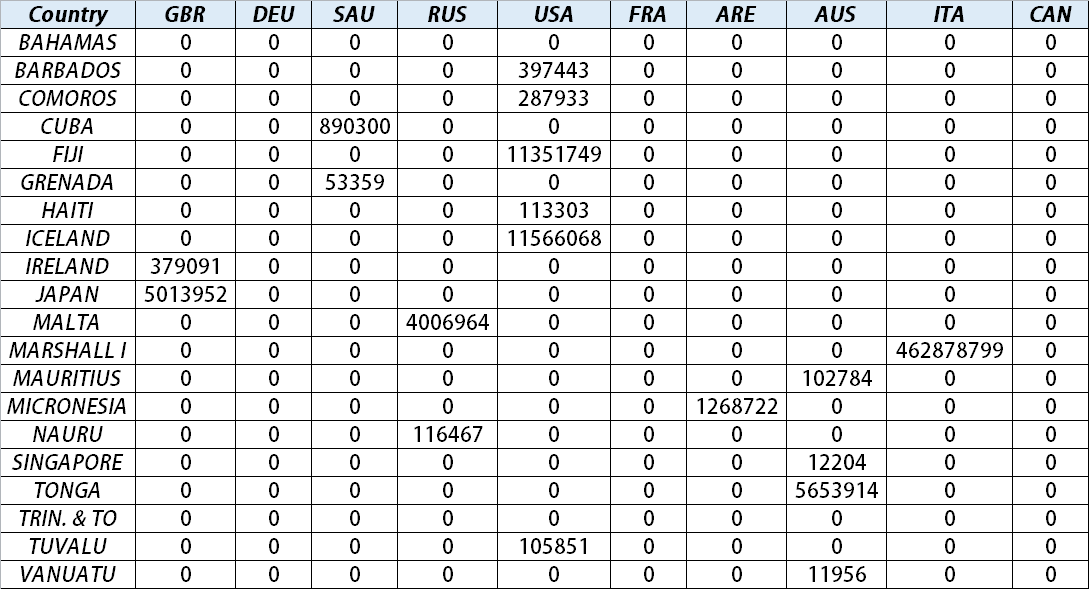
\includegraphics[width=16cm]{guihua0}%图片名
	\caption{Short-term planning (2021)}
\end{figure}
\begin{figure}[h]%
	\small
	\centering
	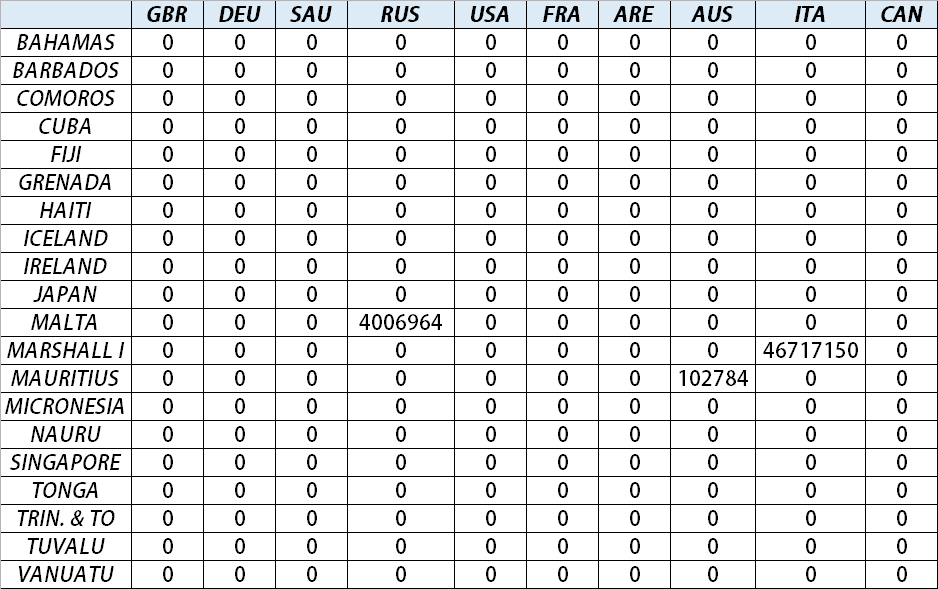
\includegraphics[width=16cm]{guihua1}%图片名
	\caption{mid-term planning (2022-2028)}
\end{figure}
\begin{figure}[h]%
	\small
	\centering
	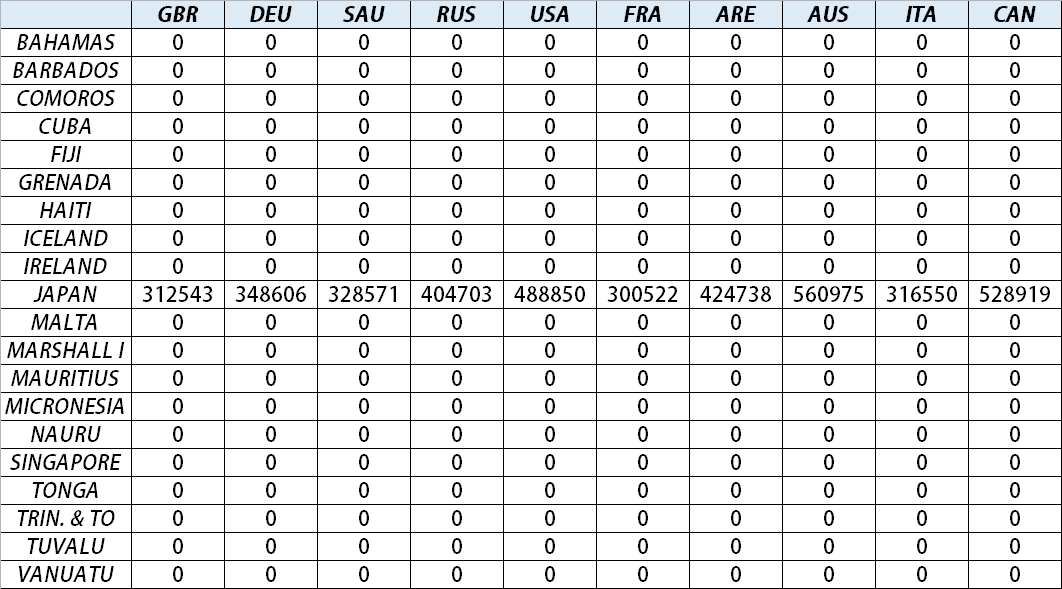
\includegraphics[width=16cm]{guihua3}%图片名
	\caption{long-term planning (2029-2050)}
\end{figure}




\end{appendices}
\end{document}
%%
%% This work consists of these files mcmthesis.dtx,
%%                                   figures/ and
%%                                   code/,
%% and the derived files             mcmthesis.cls,
%%                                   mcmthesis-demo.tex,
%%                                   README,
%%                                   LICENSE,
%%                                   mcmthesis.pdf and
%%                                   mcmthesis-demo.pdf.
%%
%% End of file `mcmthesis-demo.tex'.
